\documentclass[12pt]{article}
\usepackage[dvipsnames]{xcolor}
\usepackage{hyperref, pagecolor, mdframed }
\usepackage{graphicx, amsmath, latexsym, amsfonts, amssymb, amsthm,
amscd, geometry, xspace, enumerate, mathtools}
\usepackage{tikz}
\hypersetup{
    colorlinks=true,
    linkcolor=blue,
    urlcolor=red
}

\definecolor{wgrey}{RGB}{91, 227, 70}
\title{Module de Tate, notes 1}
\date{5 juillet 2023}
\begin{document}
\tableofcontents
\maketitle
\section{Définitions}
\indent \indent \textbf{\color{wgrey} Module de Tate} : On rappelle que (\textbf{\color{wgrey} avec choix de base})
\begin{align}
    E[l]&\cong \mathbb{Z}/l\mathbb{Z}\times\mathbb{Z}/l\mathbb{Z} \\
    E[p^e]&\cong {O}~ou~\cong \mathbb{Z}/p^e\mathbb{Z}
\end{align}
En char $p$ pour $l\ne p$. En plus, si $P\in E[l]$ et $\sigma\in Gal(\overline{k}/k)$
alors $P^{\sigma}\in E[l]$ car les polynômes à division sont définis sur $k$ si $E$ est déf sur $k$ (voir Schoof).
C'est à dire que $E[l]$ est munit d'une action de $Gal(\overline{k}/k)$ et ce sera de même pour le module de Tate.
On definit le module de Tate via : $$T_l(E)=\underset{\underset{n}{\longleftarrow}}{\textrm{lim}}~E[l]$$

Où :\\\newline
\indent \indent 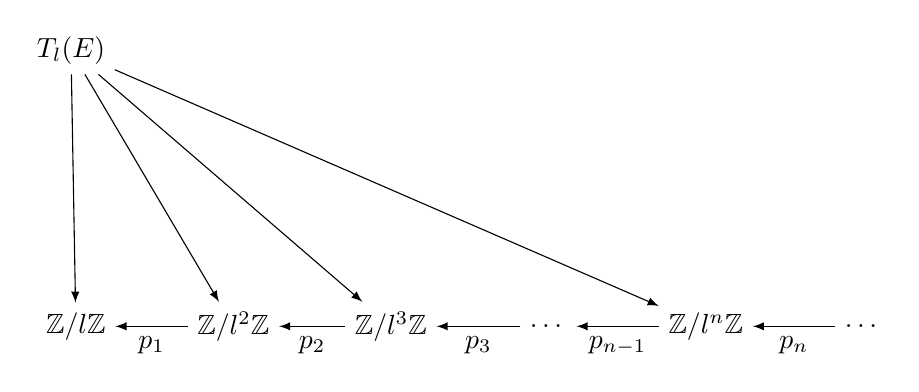
\begin{tikzpicture}[x=1cm,y=1cm,>=latex,->]
    \node(0) at (150:7) {$T_l(E)$};
    \node(1) at (180 : 6) {$\mathbb{Z}/l\mathbb{Z}$};
    \node(2) at (180 : 4) {$\mathbb{Z}/l^2\mathbb{Z}$};
    \node(3) at (180 : 2) {$\mathbb{Z}/l^3\mathbb{Z}$};
    \node(n-1) at (0 : 0) {$\dots$};
    \node(n) at (0 : 2) {$\mathbb{Z}/l^n\mathbb{Z}$};
    \node(n+1) at (0 : 4) {$\dots$};

    \foreach \k/\l in {0/1, 0/2, 0/3, 0/n}{\draw(\k)--(\l);}
    \foreach \k/\l in {1/2, 2/3, 3/n-1, n-1/n, n/n+1}{
        \draw(\l)--(\k) node[midway, below]{$p_{\k}$};
    }
\end{tikzpicture}
\\ On a via $(1)$ et $(2)$ : (\textbf{\color{wgrey} avec choix de base})
\begin{align}
   T_l(E) &\cong \mathbb{Z}_l\times\mathbb{Z}_l\\
   T_p(E) &\cong O~ou~\mathbb{Z}_p
\end{align}
Et l'action de $Gal(\overline{k}/k)$ sur $T_l(E)$ fournit une représentation : (\textbf{\color{wgrey} avec choix de base encore})

$$\rho_l~:~Gal(\overline{k}/k)\rightarrow \textrm{GL}_2(\mathbb{Z}_l)\hookrightarrow \textrm{GL}_2(\mathbb{Q}_l)$$

\noindent \textbf{\color{wgrey} On peut éviter le choix de base avec} :  
$$\rho_l~:~Gal(\overline{k}/k)\hookrightarrow \textrm{Aut}(T_l(E))\otimes_{\mathbb{Z}_l}\mathbb{Q}_l$$

\noindent Ensuite $\phi\in \textrm{Hom}(E_1, E_2)$ induit $\phi\in \textrm{Hom}(E_1[l],E_2[l])$ puis $\phi_l\in \textrm{Hom}_{\mathbb{Z}_l}(T_l(E_1), T_l(E_2))$.
\\\newline
Où en fait : \textbf{\color{ForestGreen} Le premier résultat important} 
\begin{flalign*}
    &&\textrm{Hom}(E_1, E_2)\otimes_{\mathbb{Z}}\mathbb{Z}_l\hookrightarrow\textrm{Hom}_{\mathbb{Z}_l}(T_l(E_1), T_l(E_2))&& (*)
\end{flalign*}
est une injection.\\ 
\newline
{\textbf{Preuve :}} On regarde 
\begin{itemize}
    \item $\phi$ tel que $\phi_l=0$ et $\phi\in M\otimes\mathbb{Z}_l\subset\textrm{Hom}(E_1,E_2)\otimes\mathbb{Z}_l$ un sous groupe de type fini (qui est alors libre).
    \item Et $M_{div}\otimes\mathbb{Z}_l$ (les fractions contenues dans le Hom) est alors de t.f donc libre aussi (le Hom est sans torsion). On le montre en tensorisant avec
$\mathbb{R}$. Alors $\textrm{deg}~:~M_{div}\otimes\mathbb{R}\rightarrow\mathbb{R}$ est continue et $\textrm{deg}^{-1}\big(]-\infty, 1[\big)\bigcap M_{div}\otimes\mathbb{R}=\{0\}$, i.e. $M_{div}$ est un reseau !.

Ensuite, suffit d'écrire $\phi=\sum_i \alpha_i\otimes\psi_i$ de sorte qu'on ait $\psi=\sum a_i\psi_i$ et $$a_i\equiv \alpha_i~mod~l^n$$
Alors $\phi=\lambda\circ[l^n]$ et $\lambda=\sum b_i\psi_i$ d'où $a_i=l^nb_i$ i.e. $$\alpha_i\equiv 0~mod~l^n$$
Puis $\alpha_i=0$.\qed
\end{itemize}

\textbf{Avec le choix de base et comme End($E$) est sans torsion, $$\textrm{rg}_{\mathbb{Z}}\textrm{End}(E)\leq \textrm{rg}_{\mathbb{Z}_l}\textrm{End}(T_l(E))\leq 4.$$}
\newpage
On déf $End_k(T_l(E))$ pour les endomorphismes commutant avec $Gal(\overline{k}/k)$.
\\\newline {\textbf{\color{ForestGreen} Theoreme d'Isogénie :}} L'injection $(*)_k$ est un isomorphisme quand 
\begin{itemize}
    \item $k$ est un corps de nombres. (Faltings)
    \item $k$ est un corps fini. (Tate)
\end{itemize}

Apparemment on peut voir le module de Tate comme un $H_1$ et le théorème veut alors dire qu'on cherche à savoir quand est-ce qu'un de ces morphismes
provient d'un vrai morphisme géométrique.


\end{document}